% !TEX root = ./main.tex

\section{An Overview of the Inference Process}\label{sec:overview}

\subsection{A Tour of the \NDICE Language}
We introduce the \NDICE language with an example adapted from \citet{junges2021runtime}:
A plane is approaching a runway to land, while a moving vehicle is crossing said runway. 
Naturally, the plane should not land while the vehicle is occupying the runway, and so the plane has to track the vehicle with (imprecise) sensors and estimate its position. 
Tracking moving vehicles is a common case study in probabilistic programming \cite{randone2024inference, cheng2025inference, baudart2020reactive}, and \NDICE now allows us to model the behavior of the vehicle as nondeterministic, which is not featured in other PPLs.
In particular, nondeterminism allows us to \textit{under-specify} the vehicle's behavior, as we may not be able to describe the movement of the vehicle exactly, and many (not necessarily probabilistic) factors influence how the vehicle could move. 
Hence, we use nondeterminism as an abstraction to reason about the worst case scenario, where the probability that the vehicle is on the runway when the plane lands is maximal.

We will consider a simple instance of the scenario above where the vehicle may be in three possible positions: Left of the runway (Location $0$), on the runway (Location $1$) or right of the runway (Location $2$).
At each time step, the vehicle may move one location to the right, and we take one measurement of the vehicles location with an imprecise sensor.
After three time steps, we observed the sensor measurements $0$, then $1$, and finally $2$. 
Given these measurements, we wish to determine the maximum probability that the vehicle is still on the runway after three time steps if it started at Location~$0$.
To answer this query, we model the scenario with the \NDICE program in \Cref{fig:plane}, which uses bounded numbers to represent the location of the vehicle:

\begin{wrapfigure}[19]{l}{0.5\textwidth}%
	\vspace*{-1.5\intextsep}
	\begin{center}
		\begin{tabular}{l c}
			&
			\begin{lstlisting}[language=Caml]
fun move(pos: int): int {
	let m = if nflip() then flip(0.75) 
          else flip(0.5) in 
	if m && pos != 2 then pos+1 else pos  
}

fun step(pos: int, obs: int): int {
	let new_pos = move(pos) in
	let mes = if flip(0.9) then new_pos 
            else uniform(0, 3) in
	let o = observe(mes == obs) in
	new_pos   
}

let p1 = step(0, 0) in
let p2 = step(p1, 1) in
let p3 = step(p2, 2) in
p3 == 1
\end{lstlisting}
		\end{tabular}
	\end{center}
	\vspace*{-.5em}%
	\caption{A \NDICE program to track a moving vehicle.}
	\label{fig:plane}
\end{wrapfigure}%
%
\paragraph{Vehicle Movement}
The behavior of the vehicle has both probabilistic and nondeterministic aspects:
For one, we abstract the movement speed of the vehicle with randomness, where at each time step the vehicle has either a 50\% chance or a 75\% chance to progress to the next location. 
We refer to the former as \textit{slow} and to the latter as \textit{fast}.
Furthermore, the vehicle may \enquote{decide} whether to move slow or fast at each individual time step.
However, the available information may be insufficient to model the decision process of the vehicle as a probabilistic process.
We thus model the decision process to be \textit{nondeterministic}, which allows us to bound the behavior of the vehicle across all possible strategies it could use.
In \Cref{fig:plane}, we model this behavior with the \texttt{move} function in Lines~1-5, which takes the current position of the vehicle as an argument.

In Lines 2 and 3, the variable \texttt{m} models whether the vehicle progresses to the next location. 
Here, the choice between speeds is modeled with the statement $\NFLIP$, which nondeterministically returns either true or false, and the probabilistic behavior is modeled with the statement $\FLIP\theta$, which returns $\TRUE$ with probability $\theta$ and $\FALSE$ otherwise.
Afterwards, we return the updated position of the vehicle in Line~4:
If the vehicle made progress and has not left the runway yet, then the vehicle moves to next position, otherwise it does not move.

This \textit{nondeterministic} model of the vehicle abstracts a wide range of behaviors.
For example, the vehicle could always move fast, or always slow, or it may choose randomly.
It may move fast only in the first time step, or it could pick the speed depending on the current position. 
\NDICE considers all of the aforementioned strategies, along with any combination of them. 
More precisely, our model of nondeterminism considers each context where $\NFLIP$ is called as a separate choice, where each choice can be resolved to an arbitrary probabilistic statement $\FLIP\theta$.
This allows nondeterministic choices to be made depending on previous, probabilistic outcomes and enables us to reason about a wide variety of behaviors.
In the context of \Cref{fig:plane}, this allows the ground vehicle to decide its speed individually for every location and time step.



\paragraph{Sensor Measurements}
We now consider the \texttt{step} function in Lines~7-13, which models one full time step.
To do so, \texttt{step} takes two arguments: The current real position of the vehicle \texttt{pos} and the next expected measurement \texttt{obs}.
The function first calls \texttt{move} in Line~8 to update the vehicle's position, performs the imperfect sensor measurement in Lines~9-11, and finally returns the updated position in Line~12. 
We now consider how the sensor is modeled in more detail.

First of, Lines~9-10 define how sensor measurements are derived from the real position:
With a likelihood of $90\%$ the sensor will return the correct position \texttt{new\_pos}, otherwise it returns a position uniformly at random. 
The core language of \NDICE only supports Boolean variables and choices, hence \texttt{uniform(0, 3)} is syntactic sugar for a series of coin flips, and all numbers in \Cref{fig:plane} are syntactic sugar for a tuple of Boolean values.
Thus, \NDICE is limited to \emph{bounded} numbers.

Next, notice that \texttt{mes} could randomly take any value in $\{0,1,2\}$, even though we are only interested in the behavior of the system for a fixed measurement, namely \texttt{obs}.
Thus, we use an \verb*|observe| statement in Line~11 to enforce that \texttt{mes} and \texttt{obs} are equal.
The statement \verb|observe e| enables a form of Bayesian reasoning by "removing" executions where the condition \verb*|e| does not hold.
Formally, the statement \verb|observe e| always returns $\TRUE$, but as a side effect executions where \verb*|e| is not $\TRUE$ are defined to occur with probability $0$.
After the full program has been considered, the semantics of a \NDICE program normalizes the probabilities.
This allows us to reason about the probability of a given output, conditioned by the fact that all observations succeeded.
In our example, this means we can reason about the behavior of the program, under the condition that all random measurements from Line~9 align with the expected observations.


\paragraph{The Main Expression}
As a reminder, our goal is to reason about the probability that the vehicle is at Location~$1$ after three time steps, under the condition that we observed the sensor measurements~$0$, $1$ and $2$.
This query is modeled by the main expression of the program in Lines~15-18:

Here, we can use the \texttt{step} function to model both the moving vehicle and the sensor. 
For example, the call \texttt{step(0, 0)} in Line~15 models the first time step, where the vehicle starts at Location~$0$ and we expect the sensor measurement to be $0$.
Afterwards, Lines 16 and 17 repeat this process with the next measurement and the current position of the vehicle as returned by the previous call to \texttt{step}.
Finally, the program will return $\TRUE$ in Line~18 if the vehicle is on the runway, i.e.\ at Location~$1$.


\paragraph{The Inference Query} 
Now, the \NDICE inference algorithm can determine the maximum probability that the program returns $\TRUE$, given that all \texttt{observe} statements succeed.
However, do we really need a specialized inference algorithm for nondeterminism? 
Can we not cleverly instantiate the $\NFLIP$ statement so that we can use known algorithms for purely probabilistic programs?

One option to reduce inference with nondeterminism to the purely probabilistic case is to approximate $\NFLIP$ with the a probabilistic statement $\FLIP{\frac{1}{2}}$.
However, this approach offers no bounds on the quality of the approximation, and it could lead to \textit{arbitrarily low} results compared to the intended, nondeterministic query.
Another option is to simply consider all possible ways to resolve the nondeterminism, and perform a purely probabilistic query for each of them.
This is sound, but not feasible in practice.
Even if we restrict ourselves to enumerating deterministic behaviors, meaning nondeterminism is never resolved to a random choice, this still results in an exponential amount of queries.
Namely, for a program with $n$ flip operations (both nondeterministic or probabilistic), this may result in up to $2^n$ purely probabilistic queries.

Hence, it is infeasible to reduce inference with nondeterminism to the purely probabilistic case, and a dedicated inference algorithm like \NDICE is needed.
For the example program in \Cref{fig:plane}, \NDICE is able to automatically infer that the maximum probability that the vehicle is still on the runway after the observed sequence of measurements is about $3.6 \%$.



\subsection{Non-Compositionality of Probabilistic Inference with Nondeterminism}\label{sec:subOpt}
Before we present our inference method, there is one more issue which makes combining nondeterminism and conditioning challenging:
Local optimal choices cannot generally be composed to a global optimal solution.
To illustrate this, consider the following \NDICE program:%
%
\smallskip%
\begin{center}
	\begin{tabular}{c}
\begin{lstlisting}[language=Caml]
if flip(0.5) then flip(0.75)
	else if nflip()
		then let obs = observe flip(0.5) in flip(0.5)
		else let obs = observe flip(0.05) in flip(0.05)
\end{lstlisting}
\end{tabular}
\end{center}%
\smallskip%
%
We first consider the if-statement from Line 2 in isolation.
Notably, the observations are independent of the output of the if statement, thus the conditioned probability to return $\TRUE$ is $\frac{1}{2}$ if \texttt{nflip} chooses~$\TRUE$, and $\frac{1}{20}$ otherwise.
Therefore, the optimal \textit{local} choice for the nondeterministic flip is $\TRUE$, but this is not the optimal \textit{global} choice.
For the program as a whole, the conditioned probability to return $\TRUE$  is $\frac{2}{3}$ if \texttt{nflip} chooses $\TRUE$, and $\frac{301}{420}\approx 0.716$ otherwise.

Intuitively, this effect occurs as \verb|flip(0.75)| yields a higher chance to return $\TRUE$ than either choice of the nondeterministic flip, hence it is better to choose $\FALSE$ in order to reduce the chance of a successful observation, which minimizes the impact of the nested if-statement on the overall conditioned distribution.
However, minimizing the impact of less productive branches is not always optimal either:
If we replace \verb|flip(0.75)| with \verb|flip(0.55)|, then the optimal choice is $\TRUE$ instead.
Thus, nondeterministic choices need to be made in the context of the whole program.
In a similar vein, \citet{olmedo2018conditioning} showed that expectation transformers, which are defined inductively on the program structure, cannot be extended to combine probabilistic conditioning and nondeterminism.


\subsection{The \NDICE Inference Algorithm}
This section illustrates the \NDICE inference process using the program in \Cref{fig:example_prog}:
The program first tosses a probabilistic and a nondeterministic coin and observes that at least one flip was true.
Then, two probabilistic coins are flipped and a boolean expression decides the program's output.

\begin{figure}
\begin{tabular}{l c r}

\begin{subfigure}{0.35\textwidth}

\begin{lstlisting}[language=Caml, mathescape]
let a = $\verb*|flip|_1$(0.3) in 
let b = $\texttt{nflip}_2$() in
let t = observe(a || b) in
let c = $\verb*|flip|_3$(0.4) in
let d = $\verb*|flip|_4$(0.2) in
(a || c) && d
\end{lstlisting}


$$ \varphi = (f_1 \lor f_3) \land f_4$$
$$\gamma = f_1 \lor f_2$$
$$\left[ f_1\colon 0.3, \; f_2\colon n, \;f_3\colon 0.4, \;f_4\colon 0.2 \right]$$


\caption{Example \NDICE program and the compiled boolean formulae}
\label{fig:example_prog}
\end{subfigure}



&
\begin{subfigure}{0.225\textwidth}
	\begin{center}
		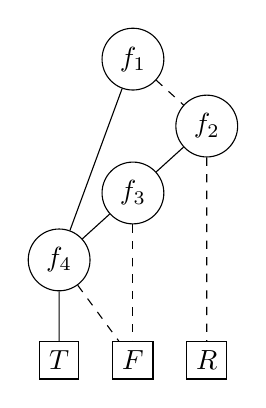
\begin{tikzpicture}[xscale=1.25, yscale=0.85]
			\node (a) at (0,0)   [draw, circle] {$f_1$};
			\node (b) at (0.75,-1)   [draw, circle] {$f_2$};
			\node (c) at (0,-2)   [draw, circle]{$f_3$};
			\node (d) at (-0.75,-3)   [draw, circle] {$f_4$};
			\node (F) at (0,-4.5)   [draw, rectangle] {$F$};
			\node (T) at (-0.75,-4.5)   [draw, rectangle] {$T$};
			\node (R) at (0.75,-4.5)   [draw, rectangle] {$R$};
			
			\path[-]          (a)  edge   [bend right=0]   node[left] {} (d);
			\path[-]          (a)  edge[dashed]   [bend right=0]   node[right] {} (b);
			
			\path[-]          (b)  edge   [bend right=0]   node[right] {} (c);
			\path[-]          (b)  edge[dashed]   [bend right=0]   node[right] {} (R);
			
			\path[-]          (c)  edge   [bend right=0]   node[right] {} (d);
			\path[-]          (c)  edge[dashed]   [bend right=0]   node[right] {} (F);
			
			\path[-]          (d)  edge   [bend right=0]   node[right] {} (T);
			\path[-]          (d)  edge[dashed]   [bend right=0]   node[right] {} (F);
		\end{tikzpicture}
	\end{center}
	\caption{Compiled ADD}
	\label{fig:example_add}
\end{subfigure}
&
\begin{subfigure}{0.375\textwidth}
	\begin{center}
	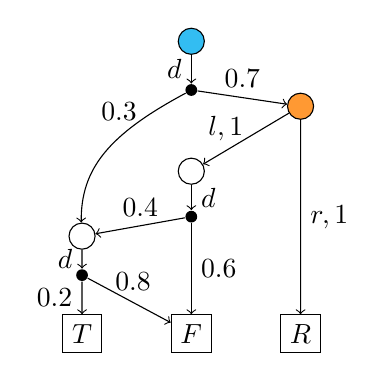
\begin{tikzpicture}[xscale=1.85, yscale=0.825]
		\node (a) at (0,0)   [draw, circle, fill=cyan!80] {$ $};
		\node (b) at (0.75,-1)   [draw, circle, fill=orange!80] {$ $};
		\node (c) at (0,-2)   [draw, circle]{$ $};
		\node (d) at (-0.75,-3)   [draw, circle] {$ $};
		\node (F) at (0,-4.5)   [draw, rectangle] {$F$};
		\node (T) at (-0.75,-4.5)   [draw, rectangle] {$T$};
		\node (R) at (0.75,-4.5)   [draw, rectangle] {$R$};

		%%%Splitting transitions start here
		\node (ao) at (0, -0.75)  [circle,fill,inner sep=1.5pt] {};
		\path[->]          (a)  edge   [bend right=0]   node[left, pos=0.5] {$d$} (ao);
		\path[->]          (ao)  edge   [bend right=20]   node[left, pos=0.15] {$0.3\;$} (d);
		\path[->]          (ao)  edge   [bend right=0]   node[above, pos=0.5] {$0.7$} (b);
		
		\path[->]          (b)  edge   [bend right=0]   node[above, pos=0.75] {$l,1$} (c);
		\path[->]          (b)  edge   [bend right=0]   node[right] {$r,1$} (R);
		
		\node (co) at (0, -2.7)  [circle,fill,inner sep=1.5pt] {};
		\path[->]          (c)  edge   [bend right=0]   node[right, pos=0.5] {$d$} (co);
		\path[->]          (co)  edge   [bend right=0]   node[above, pos=0.5] {$0.4$} (d);
		\path[->]          (co)  edge   [bend right=0]   node[right, pos=0.5] {$0.6$} (F);
		
		\node (do) at (-0.75, -3.6)  [circle,fill,inner sep=1.5pt] {};
		\path[->]          (d)  edge   [bend right=0]   node[left, pos=0.5] {$d$} (do);
		\path[->]          (do)  edge   [bend right=0]   node[left, pos=0.5] {$0.2$} (T);
		\path[->]          (do)  edge   [bend right=0]   node[above, pos=0.5] {$\;0.8$} (F);
		
	\end{tikzpicture}
\end{center}
	\caption{Final MDP}
	\label{fig:example_mdp}
\end{subfigure}

\end{tabular}
\caption{The full inference process for a \NDICE program illustrated.}
\label{fig:example_all}
\end{figure}

\paragraph{Compilation} 
The first step in the inference process is to compile two boolean formulas $\varphi$ and $\gamma$ as seen in \Cref{fig:example_prog}.
The variables in $\varphi$ and $\gamma$ correspond to flips in the original program, and so we compile a list of variables, where a variable is annotated with an $n$ if it belongs to a nondeterministic flip, and with its probability to return $\TRUE$ if it belongs to a probabilistic flip.
The formula $\varphi$ models the output of the compiled program, hence both the program and $\varphi$ return~$\TRUE$ if the first and last flip evaluate to~\TRUE.
Observations are ignored by $\varphi$, and instead $\gamma$ tracks if all observations in the compiled program would succeed.
Hence, $\gamma$ closely resembles the observation in Line 3.


\paragraph{ADD Construction}
Internally, $\varphi$ and $\gamma$ are maintained as \textit{Binary Decision Diagrams} (BDDs), and the next step combines them into the \textit{Algebraic Decision Diagram} (ADD) in \Cref{fig:example_add}.
This ADD models both the output \textit{and} observations of the compiled program, and we can evaluate it as follows:
We begin at the root, i.e. the topmost node, and assign either $\TRUE$ or $\FALSE$ to the variable $f_1$. 
If we assign $\TRUE$ to $f_1$, then we follow the solid edge to the node $f_4$, otherwise we follow the dashed edge to the node $f_2$.
We then repeat this process with the variable in the next node until we reach a terminal node. 
Notice that for any assignment to flip operations the ADD in \Cref{fig:example_add} either returns the same output as the program, or $R$ (as in \emph{R}eject or \emph{R}esample) if an observation failed.
Further, the ADD automatically removes redundant nodes, e.g. the ADD skips directly to $f_4$ when $f_1$ is $\TRUE$, as the program is unaffected by $\texttt{nflip}_2$ and $\texttt{flip}_3$ when $\texttt{flip}_1$ returns $\TRUE$.


\paragraph{Lifting to MDPs}
Next, we lift the ADD to the \textit{Markov Decision Process} (MDP) in \Cref{fig:example_mdp} by reintroducing the behavior of flips as stored by the list in \Cref{fig:example_prog}.
To do so, we lift each node in the ADD node to an MDP state, and each state's outgoing transitions are lifted from the ADD edges depending on the flip in the ADD node.
Consider for example the initial state of the MDP, which is highlighted in blue and matches to the root node of the ADD.
The root contains the variable $f_1$ which represents a probabilistic flip which is $\TRUE$ with probability $0.3$.
Thus, the MDP state has a single enabled action $d$ and branches randomly with probability $0.3$ between its successors. 
Similarly, the orange MDP state represents the ADD node with the nondeterministic flip $f_2$.
Hence, the orange state nondeterministically chooses between two actions, and each action only leads to one state.


Finally, we wish to reason about the behavior of the original program \textit{under the condition that all observations succeed}, therefore we need to consider the behavior of the MDP \textit{under the condition that R is not reached}.
This amounts to conditional reachability properties in MDPs which have been tackled in \citet{baier2014computing, junges2021runtime} by mimicking rejection sampling with an added \enquote{reset} transitions which returns executions that reach $R$ to the initial state.
However, we will be using a recently developed bisection method implemented in the Storm Model Checker~\citeBisection.
This algorithm is highly suited for our use-case, since it allows one to calculate conditional reachability probabilities very quickly on acyclic MDPs like the one we constructed in \Cref{fig:example_mdp}.

\medskip

Now, our original inference query, i.e. the maximum probability that the program in \Cref{fig:example_prog} outputs \TRUE, aligns with the maximum conditional probability to reach the state $T$ in the MDP.
But why take all these steps to build an MDP, if a valid MDP could be obtained by simply defining an operational semantics?
Simply put, the operational semantics of larger programs are too big to efficiently perform inference.
However, using ADDs as an intermediate step efficiently exploits redundancies to heavily reduce the MDP's size, which makes inference feasible for larger programs.

The use of ADDs might enable efficient inference, but this efficiency comes with the trade-off of lower expressiveness.
Namely, ADDs can only express Boolean functions, hence \NDICE is limited to programs which can be expressed with a finite amount of boolean variables.
Consequently, \NDICE is \textit{not} able to reason about unbounded numbers or continuous distributions, and programs need to be loop-free.
\Cref{sec:related_work} will later discuss tools which may not be subject to these limitations.

